\documentclass[10pt,conference]{IEEEtran}

\ifCLASSINFOpdf
	\usepackage[pdftex]{graphicx}
	%\graphicspath{{./figs/}}
	\DeclareGraphicsExtensions{.pdf,.jpeg,.png}
\else
	\usepackage[dvips]{graphicx}
	%\graphicspath{{./figs/}}
	\DeclareGraphicsExtensions{.eps}
\fi

\usepackage[cmex10]{amsmath}
\usepackage[tight,footnotesize]{subfigure}
\usepackage{xcolor}
\usepackage[lined,ruled]{algorithm2e}

\usepackage[latin1]{inputenc}
\usepackage{tikz}
\usetikzlibrary{shapes}
\usetikzlibrary{arrows}

\usepackage[]{algorithm2e}

\newtheorem{property}{Property}
\newtheorem{proposition}{Proposition}
\newtheorem{theorem}{Theorem}
\newtheorem{conjecture}{Conjecture}
\newtheorem{question}{Question}
\newtheorem{definition}{Definition}
\newtheorem{corollary}{Corollary}

\makeatletter
\pgfdeclareshape{datastore}{
\inheritsavedanchors[from=rectangle]
\inheritanchorborder[from=rectangle]
\inheritanchor[from=rectangle]{center}
\inheritanchor[from=rectangle]{base}
\inheritanchor[from=rectangle]{north}
\inheritanchor[from=rectangle]{north east}
\inheritanchor[from=rectangle]{east}
\inheritanchor[from=rectangle]{south east}
\inheritanchor[from=rectangle]{south}
\inheritanchor[from=rectangle]{south west}
\inheritanchor[from=rectangle]{west}
\inheritanchor[from=rectangle]{north west}
\backgroundpath{
    %  store lower right in xa/ya and upper right in xb/yb
\southwest \pgf@xa=\pgf@x \pgf@ya=\pgf@y
\northeast \pgf@xb=\pgf@x \pgf@yb=\pgf@y
\pgfpathmoveto{\pgfpoint{\pgf@xa}{\pgf@ya}}
\pgfpathlineto{\pgfpoint{\pgf@xb}{\pgf@ya}}
\pgfpathmoveto{\pgfpoint{\pgf@xa}{\pgf@yb}}
\pgfpathlineto{\pgfpoint{\pgf@xb}{\pgf@yb}}
 }
}
\makeatother

\newcommand{\riham}[1]{{\color{red}{#1}}}
\newcommand{\james}[1]{{\color{blue}{#1}}}


\begin{document}

\title{Exploring the reusability of the same Huffman coding tree for compressing similar data files}
\author{
\IEEEauthorblockN{Praneeth Chandra Thota}
\IEEEauthorblockA{Rutgers University\\
 Piscataway, NJ, USA\\ 
Email: pt357@rutgers.edu}
\and
\IEEEauthorblockN{Naveen Narayanan Meyyappan}
\IEEEauthorblockA{Rutgers University\\
 Piscataway, NJ, USA\\ 
 Email: nm941@rutgers.edu}
}

\maketitle
\begin{abstract}
\textnormal{
Most of the applications generate massive volumes of data and we need lot of memory to save the data. Data compression reduces the amount of data that needs to be stored and there by reduces storage costs. This project aims toward the implementation of Huffman encoding algorithm to a data set and reusing the same Huffman coding tree for the compression of similar files. Thereby we can improve the speed of compression, reduce the complexity of the algorithm and reduce the header length that is need to transmit the Huffman coding tree. In this project we will compress similar files using the conventional Huffman source coding algorithm and also using the new approach. We will then compare various charactersitics such as the compression ratios, time taken to compress and space required for compression. Eventhough this approach may not be optimal, we will still be able to acheive desirable compression at a faster rate. This new approach will be useful in cloud and edge computing applications where we have to compress the files quickly. We will tabulate the results and plot the tradeoff between speed and compression ratio for the new approach. 
}
\end{abstract}
%\onecolumn \maketitle \normalsize \vfill

\IEEEpeerreviewmaketitle
%%%%%%%%%%%%%%%%%%%%%%%%%%%%%%%%%%%%%%%%%%%%%%%%%%%%%%%%%%%%%%%%%%%%%%%%%%%%%%%%%%%%%%%%%%%%%%%%%%%%%%%%%
\section{Project Description}\label{sec:1. Project Description}
%%%%%%%%%%%%%%%%%%%%%%%%%%%%%%%%%%%%%%%%%%%%%%%%%%%%%%%%%%%%%%%%%%%%%%%%%%%%%%%%%%%%%%%%%%%%%%%%%%%%%%%%%
\textnormal{
Data compression is a reduction in the number of bits needed to represent data. Compressing data can save storage capacity, speed up file transfer, and decrease costs for storage hardware and network bandwidth. Compression is performed by a program that uses a formula or algorithm to determine how to shrink the size of the data. For data transmission, the data is compressed at the source using an algorithm and is then transmitted via the channel. The same algorithm is used to decompress the data at the receiver and the original file is retrieved.
\begin{figure}[!h]
    \centering
    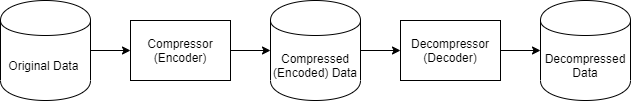
\includegraphics[width=90mm,scale=0.5]{Compressing Data.png}
    \caption{Data Compression}
\end{figure}
\linebreak
Data compression can be performed on the data content or on the entire transmission unit, including header data. When information is sent or received via the internet, larger files, either singly or with others as part of an archive file, may be transmitted in a ZIP, GZIP or other compressed format. Compressing data can be a lossless or lossy process. Lossless compression enables the restoration of a file to its original state, without the loss of a single bit of data, when the file is uncompressed. Lossless compression is the typical approach with executables, as well as text and spreadsheet files, where the loss of words or numbers would change the information. Some examples of lossless source coding algorithms are Huffman coding, Arithmetic coding and Lempel Ziv coding. Lossy compression algorithms such as Transform coding, Discrete Cosine Transform, Discrete Wavelet Transform and fractal compression algorithms permanently eliminates bits of data that are redundant, unimportant or imperceptible. Lossy compression is useful with graphics, audio, video and images, where the removal of some data bits has little or no discernible effect on the representation of the content. In this project we will explore the most commonly used lossless Huffman coding algorithm for compressing data files of similar type. Huffman coding is a fixed-to-variable length coding where in the fixed length blocks of the source output are mapped to variable length binary blocks. The main idea behind this coding is to map the more frequently occurring fixed length sequences to shorter binary sequences and the less frequently occurring sequences to longer binary sequences, thus achieving good compression ratios. In variable length coding, synchronization is a problem. This means that there should be only one way to parse the binary received sequence into code words.In other words, it is called the prefix free property: no code word can be a prefix of another code word. In this project, we will implement the Huffman encoding algorithm on a given data set and the generated encoded tree will be reused to compress other files of similar type. By this method we aim to reduce the length of the header for the data file and also the time taken to compress the file. Although the compression may not be optimal in this but we will be able to save time in compressing the data. If we are able to achieve the desirable level of compression, then this method of compression can used in applications where we are in need of the processing data at a faster rate. We will be able to save considerable amount of time and space as we will have to create the Huffman coding tree only once and we will not be required to maintain a priority queue for each data file. Moreover, we will also be able to reduce th esize of the  header file as we will not be required to transmit the Huffman coding tree which was used to compress the data. This will help us achieve more compression and better usage of the available bandwidth. In terms of running time, the original Huffman coding algorithm will have to read the data twice, once to determine the frequency/probability and the second time to encode the data. In our case, we will be reading the data only once and that is to encode the data. The other advantage of this idea is that we dont have to generate the priority queue for each data file, this will save computation time and power. Overall, this approach may not provide optimal compression ratio but it will require less computational power,space and time than the original  Hiffman coding algorithm. We will impement both the algorithms on various data sets and identify the tradeoff between the compression ratio and the time taken to compress the data.  
}

\section{Design }\label{sec:2 Design.}
%%%%%%%%%%%%%%%%%%%%%%%%%%%%%
\textnormal{
The data from a common source file is run through the Huffman source coding algorithm and the encoded tree is generated. This encoded tree is shared with the receiver for decompression. Now we will be using the same encoded tree for compressing data files of similar type.The decompressing algorithm for the file will remain the same except that we will be using the same priority queue. Moreover, we will have more compression of the header file as we will not have to send the Huffman coding tree. The following is the algorithm and flow diagram of the proposed project-
\\*
Algorithm:
\begin{enumerate}
\item{Sort source outputs in decreasing order of their probabilities/frequencies}
\item{Implement the priority queue for each charcater with their frequencies}
\item{Merge the two least probable/frequent characters/outputs from the priority into a single output by adding their corresponding probabilities/frequencies}
\item{Repeat the above step until we are left with 2 characters.The sum of probability of these two characters should be 1 and sum of their frequecies will be equal to the total number of characters in the data source}
\item{Arbitrarily assign 0 and 1 as code word for the two remaining characters/outputs from step 4}
\item{If an output is the result of the merger of two outputs in a preceding step, append the current code word with a 0 and a 1 to obtain the code word for the preceding outputs; then, repeat Step 6. If no output is preceded by the output in current step, then stop.}
\item{This will result in a Huffman coding tree which will be used to compress the data}
\item{Now use the same Huffman coding tree from step 7 to compress other data fies of similar type}
\item{All the binary files are decompressed using the same huffman coding tree generated on step 7}
\end{enumerate}
Flow Diagram:
\\*
\begin{figure}[!h]
    \centering
    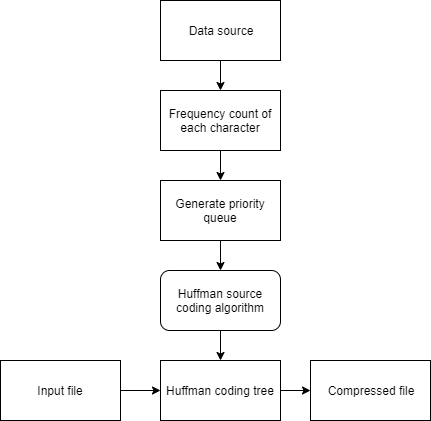
\includegraphics[width=90mm,scale=0.5]{Data Flow.png}
    \caption{Data Flow}
\end{figure}
\\*
High Level Pseudo Code System Description:
\\
procedure Huffman(f)
\begin{itemize}
  \item[] Input: An array f[1...n] of frequencies
  \item[] Output: An encoding tree with n leaves
  \item[] Let H be a priority queue of integers, ordered by f
  \item[] for i = 1 to n: 
  \item[]\makebox[0.5cm][l]{ } insert(H; i)
  \item[]for k = n + 1 to 2n - 1:
  \item[]\makebox[0.5cm][l]{ } i = deletemin(H); j = deletemin(H) 
  \item[]\makebox[0.5cm][l]{ } create a node numbered k with children i, j
  \item[]\makebox[0.5cm][l]{ } left[k] <- i
  \item[]\makebox[0.5cm][l]{ } right[k] <-j
  \item[]\makebox[0.5cm][l]{ } f[k] = f[i] + f[j]
  \item[]\makebox[0.5cm][l]{ } insert(H, k)
  \item[] return k
\end{itemize}
Here k represents the root of the Huffman coding tree with n leaves. Now we will use the same tree for compressing all data files of similar types.
\\
Data Structures:
\begin{itemize}
\item {Python Dictionary: The python dictionary stores data in a similar way as the regular dictionary. It has keys which are associated with corresponding values and these values can be referenced using the keys.}
\item {Priority Queue: A priority queue is stored in form of array/list and implemented using heaps. New values are inserted at the back and removal of values is done from the front. However, the priority of the elements is always maintained at the front and the element with the lowest priority is moved to the back.}
\end{itemize}
Complexity Analysis:
\\
Running time complexity - The conventional Huffman coding algorithm involves the calculation of frequencies for each character. For this step we need to read the entire data source once which will take time of O(n). The other time consuming step would be the deletemin and insert operations on the priority queue. Each iteration on priority queue takes O(log n). There are n iterations, one for each data point, so the overall running time complexity will be O(nlog n). In our algorithm, the first file for compression will take O(nlog n) running time, but for the subsequent files we will neithe calculate frequencies nor maintain the priority queue. Thus each character will be read from the data source and converted into binary sequences. This will take linear time to code the data.
\\
Space Complexity - The conventional algorithm requires space to maintain the priority queue for each data file. In our case this space is fixed and the stored priority queue does not change.
\\*
Constraints:
\\
It is important to note that the above proposed algorithm only works for compressing files of similar types. This is because we are using the same Hufmann coding tree generated from one common source file. While compressing a new file, if we find a new character that is not present in the Huffman coding tree then our compression algorithm will fail. So we have to be careful while choosing the data source for generating the Huffman coding tree. This data source should have all the characters that we will encounter while compressing and also the probability distribution of characters should be similar among the various input files.
\\
Timeline for the project:
\begin{itemize} 
\item{October 28th to November 2nd: Complete the description of the project} 
\item{November 2nd to November 4th: Draft a pseudo code and prepare a flow diagram for the project}
\item{November 4th to November 6th: Identifying data sets for implementing Huffman coding algorithm}
\item{November 7th to November 10th: Implementing the Huffman coding algorithm in python}
\item{November 10th to November 15th: Generate the Intermidiate report with the results so far}
\item{November 15th to November 17th: Implementing the Huffman coding algorithm on similar data sets}
\item{November 18th to November 20th: Analyse the time and space complexity and compare the compression ratios for various data sets}
\item{November 21st to November 23rd: Tabulate the results}
\item{November 24th to November 25th: Identify future extensions}
\item{November 25th to November 27th: Prepare the final report and presentation ppt, present to TA.}
\end{itemize}
Division of labor:
\begin{itemize}
\item {Praneeth: Implementation of the Huffman coding algorithm and making the presentation ppt}
\item {Naveen: Literature Review, tabulating the results and generating the reports}
\end{itemize}
}






\section{Implementation}\label{sec:3 Implementation }
%%%%%%%
\textnormal{
For implementing Hufmann source coding algorithm, we have used Python 3 Version 3. We implemented the algorithms on HP Pavilion Notebook with Intel(R) Core(TM) i5-6200 CPU @2.30Ghz processor, 64bit operating system and 8 GB RAM.  
\\
The data for the Huffman coding algorithm was taken from github repository and it has text document containing all characters of the Multilingual European Subsets of Unicode and some other common Unicode subsets. This file contains about 466k English words. We will refer this file as `data.txt' / master data file. This file is used to generate the Huffman encoding table for compression of all files of similar type. For our implementation we have created 10 sample files of size around 2000 bytes. All the sample files were named in sequence from `sample1'.txt to `sample10.txt'. All the above samples files were taken from [2]. This files were placed in a single folder along with the python codes and the data.txt file. We have our implementation on two python files: `Huffman\_User\_Command.ipynb' and `Huffman\_Encoding\_demo.ipynb'.
The flow charts and diagrams were created using draw.io application 
}





\section{Demo and Sample Findings}\label{sec:4 Demo and Sample Findings }
%%%%%%%
\textnormal{
We have implemented this approach using Python 3 and Jupyter Notebook. The file `Huffman\_User\_Command.ipynb' is used to compress the files based on the user commands. On running this file we have to input the master file which is used to generate the encoding table. This table is generated by calculating the frequency of each character in the master data file (`data.txt'). Then the user will have to choose the option of either compress/decompress/exit. On choosing compress/decompress the user will have to enter the file name to be compressed or decompressed. The input for the compression will have to be a text file and the file for decompression is an already compressed binary file. The code file continues to prompt the user to enter the subsequent actions to be taken. The user can exit from this application by entering exit in the console for action to be taken. After each compression or decompression we will get a status message(success/fail). If the action is successful then the code will aslo display the name of the compressed/decompressed file.
\\
The file `Huffman\_Encoding\_Demo.ipynb' file is used to show a demo and it does not take user inputs. The code is written to take the `data.txt' file and generate the encoding table. The encoding table generated is saved as a pickle object in the local folder. The encoding table contains the Huffman codes for each character in the master data file. This table is used to compress the subsequent data files for similar types. The code takes the `sample.txt' file and compresses it using the encoding table generated from `data.txt'. The encoded file is saved as `sample1\_compressed.bin', a binary file. The size of the compressed file is also displayed.The next step is to compare the compression ratio achieved using the original approach and the new approach. So now for the original method the encoding table is changed and the compression is performed again. Finally the 2 compression ratios are displayed. In this step we find that the compression ratio using the new approach is not optimal which was expected and the 2 compression ratios are not that different. Moreover the header for the file using our approach is larger than the original method.Now when we try to compress the next file `sample2.txt', the compression using our method is faster and this time we dont have to send the header. On combining the compresed file and the headers, we find that the compression using our new approach works better than the original method.
\\
One of the errors that we may encouter in our file is that if the sample file to be compressed contains a new character that was not present in the original master data file. The screenshot for which is given below:
\\*
\begin{figure}[!h]
    \centering
    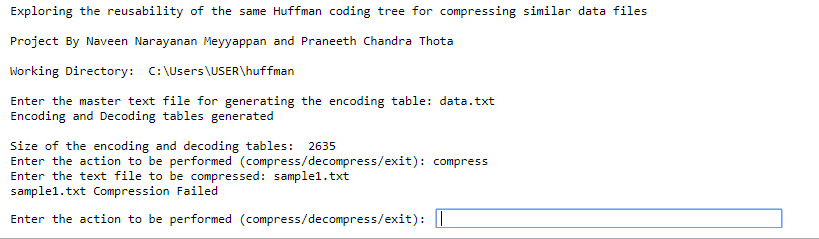
\includegraphics[width=90mm,scale=0.5]{Capture3.png}
    \caption{Error Message}
\end{figure}
\\*
\\On compressing the 10 sample files using the 2 methods we found that the total size of the compressed files including the headers using the original approach is 38627 bytes and 34012 bytes using the new approach. On the whole we have achieved higher compression and also the compression using our method is faster. Thereby we conclude that this method serves as a faster alternative for the original huffman compression. Moreover this method reduces the time and complexity of the algorithm.
}

\section{Challenges}\label{sec:5 Challenges. }
%%%%%%%
\textnormal{
The biggest challenge while implementing this project is, coming across the character that is already not present in the encoded tree. We can overcome this challenge by, 
\begin{itemize}
    \item{Choosing a data set with wide range of characters involved.}
    \item{Whenever a new character is identified the encoded tree can be modified, this method may seem little redundant but in long run it will be efficient. We assume that for each new input at least one new character is identified. As the number of inputs are increased the character range of tree will also be increased. }
\end{itemize}
} 
\section{Future Extensions}\label{sec:6 Future Extensions. }
%%%%%%%
\textnormal{
The possible future extensions for this project would be - 
\begin{itemize}
\item{One of the failures for the above approach is that this algorithm will fail when we encounter new characters that are not present in the Huffman coding tree. This problem can be solved taking an adaptive approach to the Huffman coding where in a new Huffman coding tree will be generated as when a new character is encountered in the data files. This will reduce the complexity of identifying a data file with all the characters for generating the Huffman coding tree.}
\item{Another possbile extension for this approach would be to improve the compression ratio in the above approach. This can be done creating more than one Huffman coding trees. These trees should have a significant difference in their distributions. Then we can compress our new file with all the trees and use the tree that gives us less compression ratio. Eventhough this method may not give us optimal compression but it will give a considerable amount of compression for most of the input files without increasing the running time complexity}
\end{itemize}
}
\section{References}\label{sec:7 References. }
%%%%%%%
\begin{enumerate}
\item{David A. Huffman, ``A Method for the Construction of Minimum-Redundancy Codes*", Proceedings of the I.R.E}
\item{Thomas H. Cormen, Charles E. Leiserson, Ronald L. Rivest, Clifford Stein,``Introduction to Algorithms" Second Edition, The MIT Press, Mcgraw Hill Book Company,2002. Chapter 16 - Greedy Algorithms, Pg 370}
\item{S. Dasgupta, C. H. Papadimitriou, and U. V. Vazirani, ``Algorithms", 2006, Chapter 5, Greedy Alforithms, Pg 133}
\item{B.P. Lathi, ``Modern Digital and Analog Communication Systems", 3rd Edition, Oxford Press, 2007, Chapter 16 - Introduction to Information Theory, pg 679}
\item{J.G. Proakis, M. Salehi. ``Fundamentals of Communication Systems", Pearson Education, 2006, Chapter 12 - An Introduction to Information Theory, pg 641}
\item{https://searchstorage.techtarget.com/definition/compression}
\item{Gadiel Seroussi, Marcelo Weinberger, ``Lossless Source Coding", https://www.cs.purdue.edu/homes/spa/courses /msri04/ datacomppart1.pdf}
\item{Mamata Sharma, ``Compression Using Huffman Coding", IJCSNS International Journal of Computer Science and Network Security, Vol.10 No.5, May 2010 } 
\end{enumerate}

\end{document}



